\section{Documentazione}

Di seguito sono descritte le norme che i membri del gruppo SWEnergy devono
seguire per la creazione e la modifica dei documenti. La prima sotto-sezione
riguarda l'algoritmo adottato dal gruppo per la creazione e il rilascio di un
documento in modo sintetico. Le sezioni s\gls{UC}$^G$cessive approfondiscono, descrivono
e motivano le scelte effettuate dal gruppo per la creazione e la modifica dei
documenti.

\subsection{Riassunto della creazione e del rilascio di un documento}

\begin{enumerate}
	\item Creazione della cartella del documento nella \textit{\gls{Repository}$^G$}
	      \href{https://\gls{\gls{Git}$^G$Hub}.com/Project-SWEnergy/doc-latex}{\texttt{doc-latex}}.
	\item Creazione del documento con i \textit{template} descritti in
	      sezione \S\ref{documentazione_versionamento}.
	\item Creazione del registro delle modifiche.
	\item Inserimento delle variabili del documento nel file
	      \texttt{main.tex} che si trova nella cartella del documento.
	\item Creazione delle sezioni del documento.
	\item Verifica del documento con conseguenti correzioni e avanzamento di
	      versione.
	\item Approvazione del documento con conseguenti correzioni e avanzamento
	      di versione.
\end{enumerate}

La pubblicazione di un documento avviene in due modi:
\begin{itemize}
	\item \textbf{Verbali esterni}: il verificatore dovrà inserire il documento
	      nella \textit{\gls{Repository}$^G$}
	      \begin{sloppypar}
		      \href{https://\gls{\gls{Git}$^G$Hub}.com/Project-SWEnergy/Project-SWEnergy.\gls{\gls{Git}$^G$Hub}.io}{\texttt{Project-SWEnergy.\gls{\gls{Git}$^G$Hub}.io}}
		      nel percorso \texttt{verbali\_esterni}.
	      \end{sloppypar}
	\item \textbf{Altri documenti}: il documento verrà pubblicato in automatico
	      nella \textit{\gls{Repository}$^G$}
	      \begin{sloppypar}
		      \href{https://\gls{\gls{Git}$^G$Hub}.com/Project-SWEnergy/Project-SWEnergy.\gls{\gls{Git}$^G$Hub}.io}{\texttt{Project-SWEnergy.\gls{\gls{Git}$^G$Hub}.io}}
		      attraverso l'azione di \textit{\gls{\gls{Git}$^G$Hub} Actions}.
	      \end{sloppypar}
\end{itemize}

\subsection{Strumenti}
Gli strumenti utilizzati per la creazione dei documenti sono:
\begin{itemize}
	\item \textbf{LaTeX}: linguaggio di \textit{markup} per la creazione di documenti \\
	      \href{https://www.latex-project.org/}{(www.latex-project.org)};
	\item \textbf{VisualStudio Code}: GUI con integrazioni per la creazione di documenti scritti in LaTeX e per la gestione delle \gls{Repository}$^G$ \gls{Git}$^G$ \\
	      \href{https://code.visualstudio.com/}{(code.visualstudio.com)}
	      \begin{itemize}
		      \item \textbf{LaTeX Workshop}: estensione utilizzata in VisualStudio Code per la compilazione e la scrittura dei documenti.
	      \end{itemize}
\end{itemize}


\subsection{Creazione e modifica di un documento}

A ciascun documento corrisponde un'omonima cartella che viene creata nella
\textit{\gls{Repository}$^G$}
\href{https://\gls{\gls{Git}$^G$Hub}.com/Project-SWEnergy/doc-latex}{\texttt{doc-latex}}
presente su \gls{\gls{Git}$^G$Hub}. Il nome della cartella corrisponde al nome del documento che
deve avere la prima lettera maiuscola, sono previsti gli spazi tra le parole e
le parole s\gls{UC}$^G$cessive alla prima sono in minuscolo.
La cartella di ciascun documento ha la seguente struttura:

\dirtree{%
	.1 / (Nome del documento).
	.2 main.tex.
	.2 sec.
	.3 registro\_modifiche.tex.
	.3 introduzione.tex.
	.3 le\_altre\_sezioni.tex.
}

\subsection{\textit{Template} dei documenti}

Di seguito sono elencati i \textit{template} che devono essere importati da
ciascun documento:
\begin{itemize}
	\item \textbf{Copertina}: il primo \textit{template} importato da ogni
	      documento è la copertina, che formatta la prima pagina del documento;
	      ciasun documento deve definire i comandi necessari per la costruzione
	      della copertina.

	\item \textbf{Header e footer}: ciascun documento deve importare il file
	      \texttt{header\_footer.tex} che definisce l'header e il footer di ogni
	      pagina del documento.

	\item \textbf{Variabile}: ciascun documento deve importare il file
	      \texttt{variable.tex} che definisce i comandi per la definizione delle
	      variabili globali tra i documenti; per esempio il nome del gruppo o la
	      mail del gruppo.

	\item \textbf{\textit{Template ad hoc}}: qualche documento potrebbe avere
	      dei comandi specifici per la propria creazione e stesura; per esempio,
	      l'"Analisi dei requisiti" ha bisogno di un comando per la creazione di
	      un \gls{Caso d'uso}$^G$.
\end{itemize}
Ogni documento creato dovrà quindi importare al suo interno i \textit{template}
appena descritti.
Nota bene, ogni documento include i \textit{template} sopra descritti con la
seguente sintassi:
\begin{lstlisting}[language=TeX]
	\documentclass[a4paper, 12pt]{article}
	\newcommand{\template}{../../templates}
	\usepackage{\template/package}
	\graphicspath{{../../assets}}

	\newcommand{\Titolo}{Norme di progetto}
	% ... altre variabili

	\newcommand{\Gruppo}{SWEnergy}
\newcommand{\Mail}{\href{mailto:project.swenergy@gmail.com}{project.swenergy@gmail.com}}

\renewcommand\familydefault{\sfdefault} % Set default font family to sans-serif
\linespread{1.5}

\hypersetup{
	pdfmenubar=true,            % show Acrobat’s menu?
	pdfstartview={FitH},        % fits the width of the page to the window
	colorlinks=true,            % false: boxed links; true: colored links
	linkcolor=black,            % color of internal links (change box color with linkbordercolor)
	% citecolor=green,          % color of links to bibliography
	% filecolor=magenta,        % color of file links
	urlcolor=[RGB]{156,1,198}   % color of external links
}

	\newcommand{\copertina}{
	\begin{titlepage}
		\vspace*{-3.5cm}
		\makebox[\textwidth]{
\includegraphics[width=\paperwidth]{header.png}}
		\begin{center}
			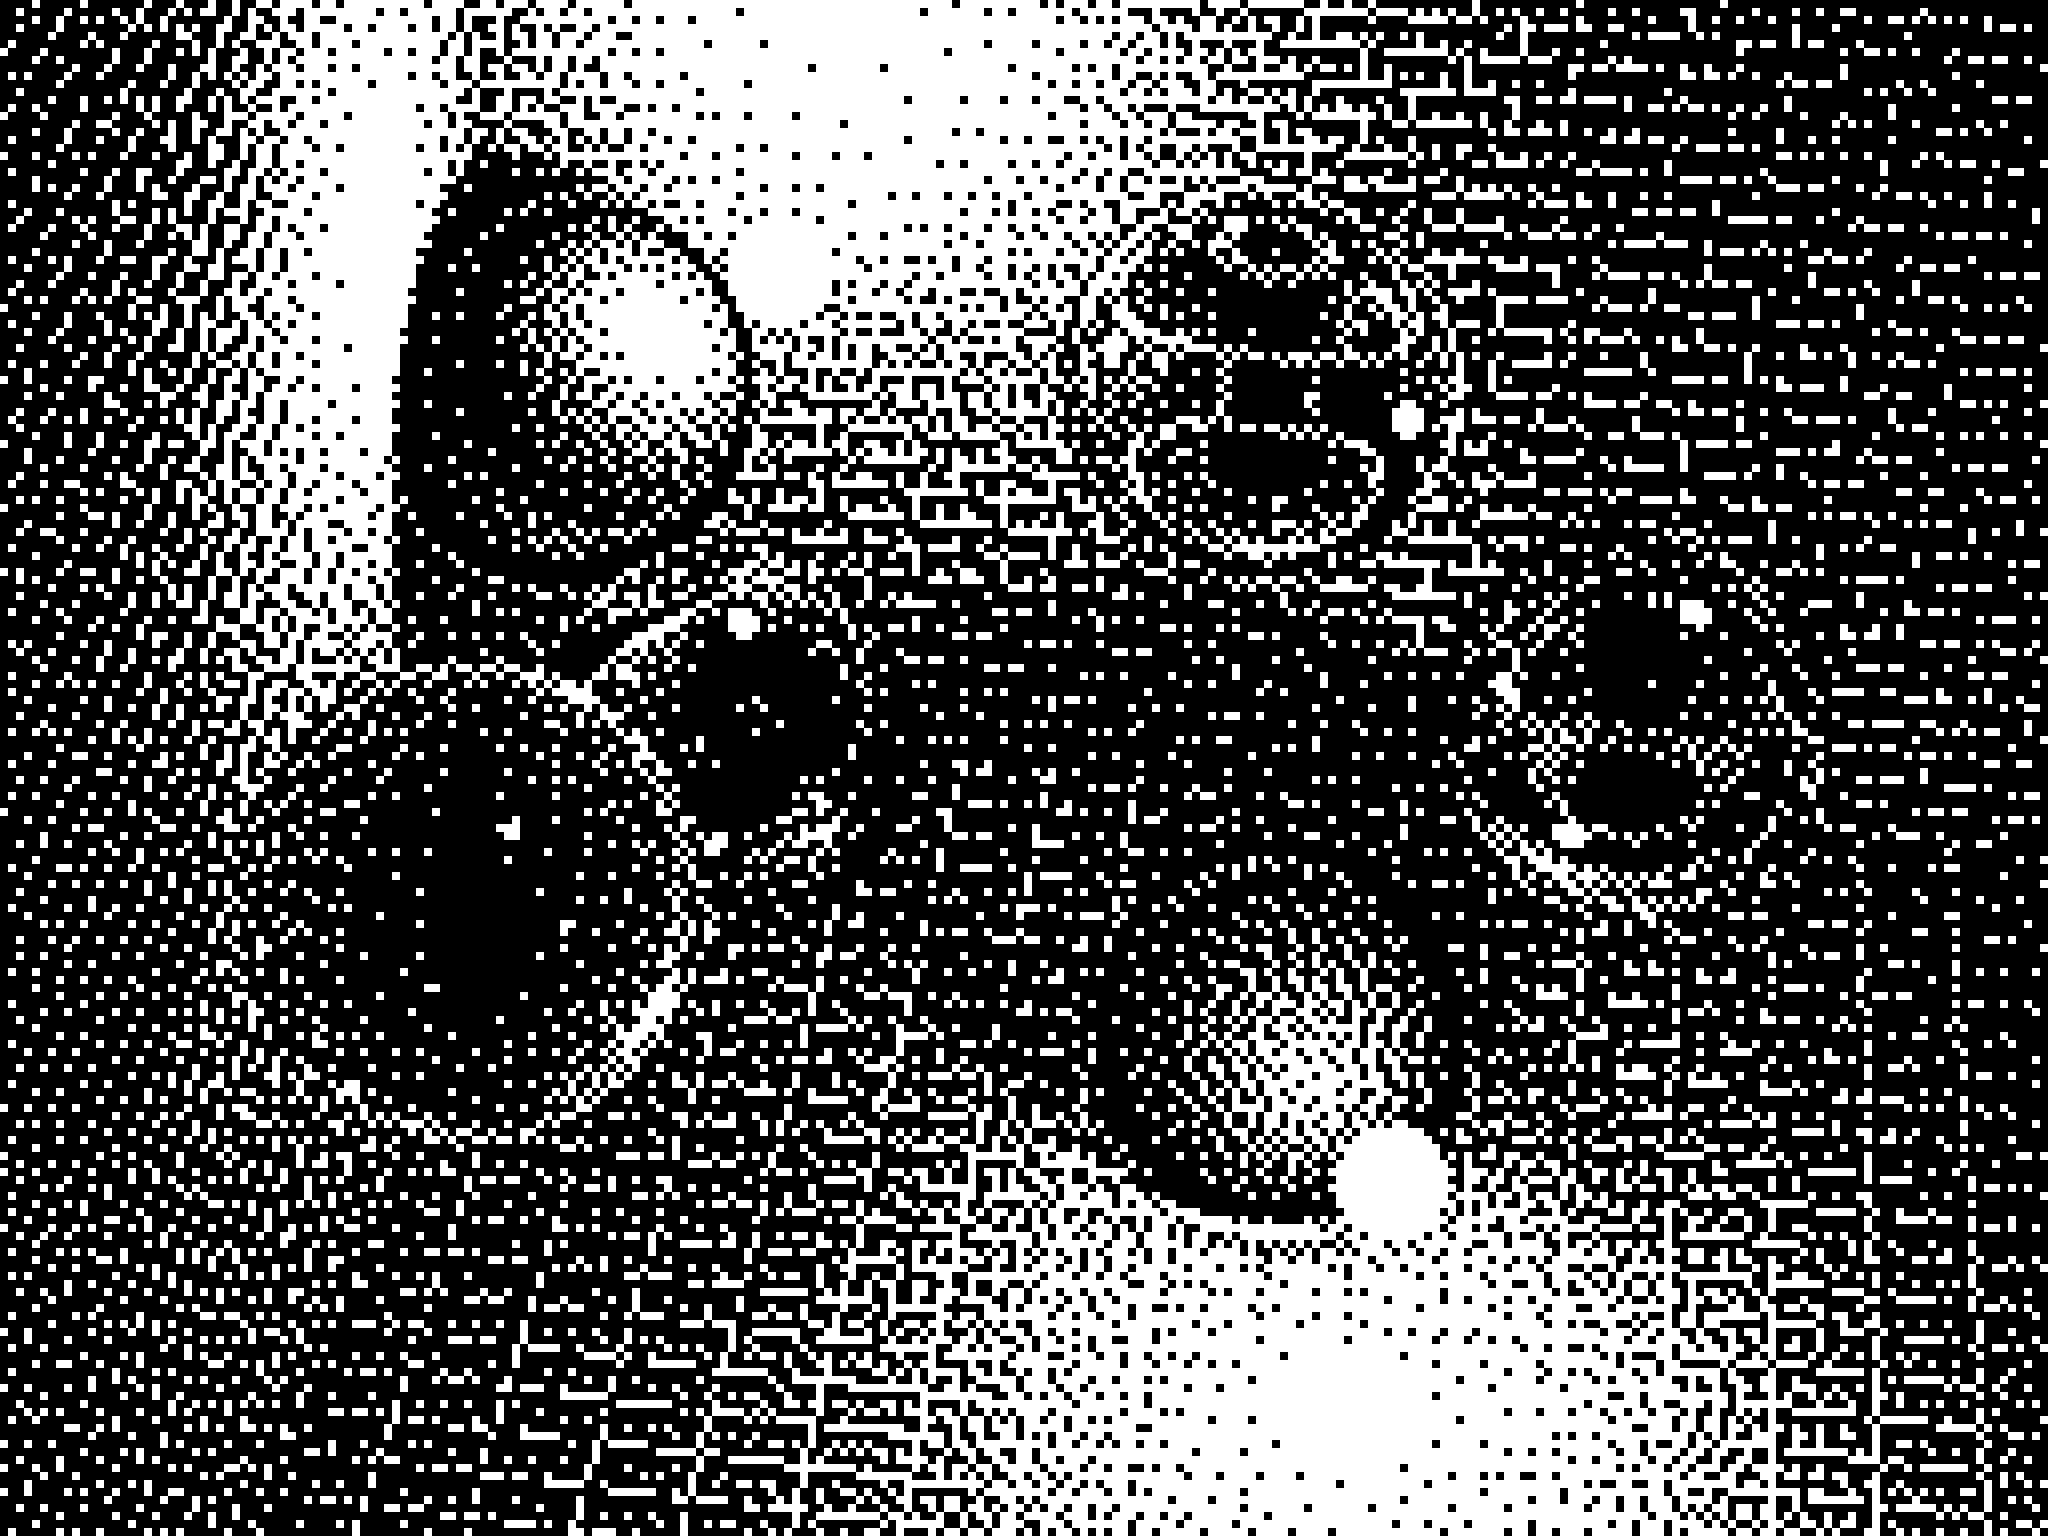
\includegraphics[width=1\textwidth]{logo.png}	\\
			\vspace{1cm}
			\Mail	\\
			\vspace{0.5cm}
			\textbf{\begin{LARGE} \Titolo \end{LARGE}}		\\
			\vspace{1cm}
			\textbf{Descrizione:} \Descrizione{}			\\
			\vspace{1cm}
			\begin{tabular}{ll}
				\textbf{Stato}               & \Stato              \\
				\textbf{Data}                & \Data               \\
				\midrule
				\textbf{Redattori}           & \Redattori          \\
				\textbf{Verificatori}        & \Verificatori       \\

				\ifdefined\Approvatori
				\textbf{Approvatori}         & \Approvatori        \\
				\fi

				\ifdefined\ApprovatoriInterni
				\textbf{Approvatori interni} & \ApprovatoriInterni \\
				\fi

				\ifdefined\ApprovatoriEsterni
				\textbf{Approvatori esterni} & \ApprovatoriEsterni \\
				\fi

				\ifdefined\Destinatari
				\textbf{Destinatari}         & \Destinatari        \\
				\fi

				\midrule

				\ifdefined\Versione
				\textbf{Versione}            & \Versione           \\
				\fi
			\end{tabular}
		\end{center}
		\vspace{4cm}
	\end{titlepage}
	\newpage
}

	\fancypagestyle{plain}{
	\fancyhf{}
	\rhead{ 
\includegraphics[scale=0.05]{horizontal_logo.png}}
	\lhead{\Titolo \ifdefined\Versione \ \Versione \fi}
	%\lfoot{\Titolo}
	\rfoot{\thepage{} di \pageref{LastPage}}
	\renewcommand{\headrulewidth}{0.2pt}
	\renewcommand{\footrulewidth}{0.2pt}
}
\pagestyle{plain}

	% ... altri template
\end{lstlisting}

In questo modo è possibile mantenere uniforme la struttura di tutti i
documenti e semplificarne la creazione.

\subsection{Variabili dei documenti}

Ciascun documento deve definire alcune variabili che sono utilizzate per
costruirne la struttura e la copertina. Di seguito sono elencate le variabili da
definire per ciascun documento:
\begin{itemize}
	\item \textbf{Verbale interno}:
	      \begin{itemize}
		      \item \textbf{Titolo}: "Verbale interno".
		      \item \textbf{Data}: la data in cui ha avuto luogo la riunione.
		      \item \textbf{Versione}: la versione del verbale.
		      \item \textbf{Descrizione}: una breve descrizione del verbale.
		      \item \textbf{\gls{Stato}$^G$}: lo \gls{Stato}$^G$ del verbale, ovvero se è \gls{Stato}$^G$
		            approvato o meno.
		      \item \textbf{Redattori}: i redattori del verbale (in genere è il
		            responsabile).
		      \item \textbf{Verificatori}: i verificatori del verbale (in genere
		            è il verificatore).
	      \end{itemize}

	\item \textbf{Verbale esterno}:
	      \begin{itemize}
		      \item \textbf{Titolo}: "Verbale esterno - Imola Informatica".
		      \item \textbf{Data}: la data in cui ha avuto luogo la riunione.
		      \item \textbf{Versione}: la versione del verbale;
		      \item \textbf{Descrizione}: una breve descrizione del verbale.
		      \item \textbf{\gls{Stato}$^G$}: lo \gls{Stato}$^G$ del verbale, ovvero se è \gls{Stato}$^G$
		            approvato o meno.
		      \item \textbf{Redattori}: i redattori del verbale (in genere è il
		            responsabile).
		      \item \textbf{Verificatori}: i verificatori del verbale (in genere
		            è il verificatore).
		      \item \textbf{Approvatori esterni}: i nomi degli approvatori
		            esterni, ovvero dei proponenti.
	      \end{itemize}

	      Nota bene, ciascun verbale esterno deve essere firmato dai proponenti,
	      per questo motivo è necessario inserire uno spazio apposito alla fine
	      del documento attraverso il comando \texttt{\\firma\{\}} definito nel
	      \textit{template} \texttt{firma.tex}.

	\item \textbf{Documenti generici}:
	      \begin{itemize}
		      \item \textbf{Titolo}: il nome del documento.
		      \item \textbf{Data}: la data di creazione del documento.
		      \item \textbf{Versione}: la versione del documento.
		      \item \textbf{Descrizione}: una breve descrizione del documento.
		      \item \textbf{\gls{Stato}$^G$}: lo \gls{Stato}$^G$ del documento, ovvero se è \gls{Stato}$^G$
		            approvato o meno.
	      \end{itemize}

\end{itemize}


\subsection{Versionamento}
\label{documentazione_versionamento}
Ogni documento rilasciato dovrà presentare un versionamento interno indicato con
tre interi positivi nel formato \texttt{X.Y.Z}, dove:
\begin{itemize}
	\item \textbf{X}: da incrementare in di rilascio di un
	      documento, indica l'ultima versione ufficialmente rilasciata.
	      L'incremento di questa cifra comporta l'azzeramento delle cifre Y e Z
	      e avviene con modalità differenti a seconda del documento.

	\item \textbf{Y}: da incrementare in caso avvenga la verifica e
	      l'approvazione di un documento; indica il numero di verifiche
	      effettuate sul documento. L'incremento di questa cifra comporta
	      l'azzeramento della cifra Z.

	\item \textbf{Z}: da incrementare in caso avvenga modifica, creazione o
	      eliminazione di una qualunque porzione di testo del documento; indica
	      il numero di modifiche effettuate sul documento.
\end{itemize}

Ogni documento dovrà essere creato partendo dalla versione \texttt{0.0.1}, ogni
s\gls{UC}$^G$cessivo incremento alla versione dovrà essere accompagnato da una nuova riga
nella tabella "Registro delle modifiche" che espliciti i cambiamenti effettuati.
Modifiche quali correzioni grammaticali o leggere variazioni nel testo non vanno
riportate nel registro delle modifiche e non prod\gls{UC}$^G$ono un avanzamento di
versione.
La verifica di un documento comporta l'incremento della cifra Y, mentre
L'approvazione di un documento avviene solo quando il documento deve essere
rilasciato.

\subsection{Verifica di un documento}
Ogni documento deve essere necessariamente verificato da un Verificatore, il
quale si occuperà di revisionare i seguenti aspetti:
\begin{itemize}
	\item Correttezza grammaticale.
	\item Correttezza logica.
	\item Correttezza e completezza del contenuto in modo che risulti coerente
	      con il documento.
	\item Adesione al \textit{Way of Working}.
\end{itemize}
\noindent
In caso il verificatore dovesse riscontrare dei problemi questi vanno segnalati
su \gls{\gls{Git}$^G$Hub} tramite i commenti presenti all'interno dell'apposita sezione
"Pull Request".
Questa azione genera una notifica immediata al red\gls{Attore}$^G$, il quale provvederà
ad apportare le modifiche necessarie. \\
In caso invece il documento non richieda modifiche si dovrà procedere ad un
avanzamento di versione come descritto in sezione
\S\ref{documentazione_versionamento}.


\subsection{Approvazione di un documento}
L'approvazione di un documento avviene solo quando il documento deve essere
rilasciato. A seconda del documento, l'approvazione interna è svolta in modo
diverso:
\begin{itemize}
	\item \textbf{Verbali}: un verbale viene approvato quando un verificatore
	      ritiene che il documento sia pronto per il rilascio.

	\item \textbf{Altri documenti}: l'incremento di questa cifra avviene
	      quando due verificatori ritengono che il documento sia pronto per il
	      rilascio.
\end{itemize}

Ogni documento approvato deve subire un avanzamento di versione come descritto
alla sezione \S\ref{documentazione_versionamento}.
\noindent
In caso il documento in questione sia un verbale esterno, il verificatore dovrà
occuparsi di effettuare una approvazione interna e, s\gls{UC}$^G$cessivamente, inviare il
documento in allegato ad una \textit{email} al fine di ottenere l'approvazione
esterna del verbale. Una volta firmato il documento, il verificatore dovrà
inserire il documento nella \textit{\gls{Repository}$^G$}
\href{https://\gls{\gls{Git}$^G$Hub}.com/Project-SWEnergy/Project-SWEnergy.\gls{\gls{Git}$^G$Hub}.io}{\texttt{Project-SWEnergy.\gls{\gls{Git}$^G$Hub}.io}}
nella cartella \texttt{verbali\_esterni}.


\subsection{Struttura dei verbali interni}

I verbali interni sono suddivisi in 4 porzioni, in \gls{Ordine}$^G$:
\begin{itemize}
	\item \textbf{\gls{Partecipanti}$^G$}: in questa sezione è indicata la durata della
	      riunione. Di seguito è presente una tabella che indica i nomi dei
	      componenti di SWEnergy, il loro ruolo e la durata della partecipazione
	      alla riunione.

	\item \textbf{\gls{Ordine}$^G$ del giorno}: in questa sezione è presente una lista
	      dei punti che sono stati discussi durante la riunione e le pagine nel
	      quale sono trattati. Si noti che questa sezione è generata
	      automaticamente e corrisponde alla tabella dei contenuti.

	\item \textbf{Sezioni di approfondimento}: sono presenti più sezioni che
	      spiegano ciascuno dei punti dell'\gls{Ordine}$^G$ del giorno. La prima di queste
	      sezioni deve essere il \textit{Brainstorming} che rappresenta il
	      resoconto delle attività svolte nell'ultimo mini-\textit{sprint}.

	\item \textbf{Assegnazione degli incarichi}: in questa sezione sono
	      presenti gli incarichi assegnati ai vari componenti del gruppo, viene
	      anche indicata la \textit{\gls{Issue}$^G$} di \gls{\gls{Git}$^G$Hub} di riferimento se presente.
\end{itemize}

\subsection{Struttura dei verbali esterni}
I verbali esterni hanno una struttura simile a quella dei verbali interni, ma
sono presenti alcune differenze:
\begin{itemize}
	\item \textbf{\gls{Partecipanti}$^G$}: in questa sezione è indicata la durata della
	      riunione. Di seguito è presente una tabella che indica i nomi dei
	      componenti di SWEnergy, il loro ruolo e la durata della partecipazione
	      alla riunione. In questa tabella viene anche inserito il nome dei
	      proponente presenti alla riunione.

	\item \textbf{\gls{Ordine}$^G$ del giorno}: questa sezione è identica a quella dei
	      verbali interni. Ovvero, è presente una lista dei punti che sono stati
	      trattati durante il \textit{meeting} e le pagine nel quale sono
	      approfonditi gli argomenti. Questa pagina è generata automaticamente
	      e corrisponde alla tabella dei contenuti.

	\item \textbf{Sezioni di approfondimento}: questa sezione è identica a
	      quella dei verbali interni. Ovvero, sono presenti più sezioni che
	      spiegano ciascuno dei punti dell'\gls{Ordine}$^G$ del giorno. La prima di queste
	      sezioni deve essere il \textit{Brainstorming} che rappresenta il
	      resoconto delle attività svolte nell'ultimo mini-\textit{sprint}.

	\item \textbf{Conclusioni}: in questa sezione sono presenti le conclusioni
	      del \textit{meeting} e le decisioni prese. In particolare, in questa
	      sezione sono chiariti gli impegni presi dal gruppo che dovranno essere
	      risolti entro la prossima riunione.
\end{itemize}

\subsection{Struttura dei documenti generici}

Poiché i documenti generici sono molto diversi tra loro e sono unici, non è
trattata la descrizione della loro struttura. Piuttosto, si richiede che in ogni
documento sia presente un'introduzione che ne descriva lo scopo e la struttura.
Di seguito sono riportati gli elementi comuni a tutti i documenti generici che
devono essere presenti:
\begin{itemize}
	\item \textbf{Registro delle modifiche}:
	      Ogni documento, esclusi verbali e presentazione, include subito dopo
	      la copertina un registro delle modifiche in forma tabellare, come
	      indicato nei riferimenti. Vi sono le seguenti voci:
	      \begin{itemize}
		      \item \textbf{Versione}: indica da versione del documento alla
		            riga di modifica.
		      \item \textbf{Data}: indica la data di redazione, verifica o
		            approvazione.
		      \item \textbf{Red\gls{Attore}$^G$}: nome del componente del gruppo che ha
		            effettuato la redazione.
		      \item \textbf{Verificatore}: nome del componente del gruppo che ha
		            effettuato la verifica.
		      \item \textbf{Approvatore}: nome del componente del gruppo che ha
		            effettuato l'approvazione.
		      \item \textbf{Descrizione}: breve descrizione della sezione
		            oggetto di redazione e verifica, in caso di approvazione
		            indica l'azione svolta e la fase di avanzamento attuale.
	      \end{itemize}
	      \noindent
	      La tabella viene riportata in \gls{Ordine}$^G$ decrescente di modifica, così da
	      mantenere sempre in cima le azioni più recenti eseguite.

	\item \textbf{Indice}:
	      Ogni documento include subito dopo il registro delle modifiche un
	      indice che elenca le sezioni del documento. L'indice è generato
	      automaticamente e corrisponde alla tabella dei contenuti.

	\item \textbf{Introduzione}:
	      Ogni documento include, subito dopo l'indice, un'introduzione che
	      descrive lo scopo del documento e la struttura del documento stesso.
	      Ciascuna introduzione deve contenere le seguenti sotto-sezioni:
	      \begin{itemize}
		      \item \textbf{Scopo del documento}: descrive lo scopo del
		            documento.
		      \item \textbf{Scopo del prodotto}: descrive lo scopo del prodotto
		            che si andrà a realizzare.
		      \item \textbf{Glossario}: contiene i termini che necessitano di
		            ulteriore contestualizzazione o che necessitano di essere
		            chiariti.
		      \item \textbf{Riferimenti}: contiene i riferimenti utilizzati
		            durante la stesura del documento, sia interni che esterni.
	      \end{itemize}
\end{itemize}

\subsection{Diario di bordo}

Il diario di bordo è una presentazione \textit{PowerPoint} che viene mostrata
al committente ad intervalli regolari. I diari di bordo si trovano nella
cartella \texttt{diario\_di\_bordo} su \textit{Google Drive}, nell'account del
gruppo SWEnergy.

\subsection{Creazione del diario di bordo}

Per creare il diario di bordo è necessario seguire i seguenti passi:
\begin{enumerate}
	\item Si visualizza un diario di bordo precedente.
	\item Si effettua una copia del diario di bordo precedente.
	\item Si aggiorna la prima diapositiva con le informazioni della nuova
	      riunione.
	\item Si aggiornano gli header con la data della nuova riunione.
	\item Si aggiorna la seconda diapositiva con le attività svolte e i problemi
	      riscontrati.
	\item Si aggiorna la terza diapositiva con le attività da svolgere e i dubbi
	      inerenti.
\end{enumerate}

In ogni caso, il diario di bordo deve essere creato in una riunione di gruppo
precedente alla riunione con il committente. In particolare, il diario di bordo
deve essere creato in seguito alla retrospettiva del mini-\textit{sprint}.

\subsubsection{Struttura del diario di bordo}

In ciascuna diapositiva devono essere presenti
\begin{itemize}
	\item \textbf{Logo}: il logo del gruppo in basso a sinistra.
	\item \textbf{Numero diapositiva}: il numero della diapositiva in basso a
	      destra rispetto al numero totale di diapositive.
	\item \textbf{\textit{Header}}: ":\textbackslash{}Università
	      degli Studi di Padova\textbackslash{}Diario di bordo\textbackslash{}"
	      più la data della riunione nel formato "GG\_MM\_AAAA".
\end{itemize}

Ogni diario di bordo è composto da 4 diapositive, in \gls{Ordine}$^G$:
\begin{enumerate}
	\item \textbf{Introduzione}: contiene il logo del gruppo e il nome del
	      gruppo. In aggiunta, contiene il nome del documento, la città in cui è
	      tenuta la riunione e la data della riunione.

	\item \textbf{Brainstorming}: contiene il resoconto delle attività svolte
	      dall'ultimo diario di bordo e i problemi riscontrati duranto lo
	      svolgimento delle attività.

	\item \textbf{Pianificazione}: contiene la pianificazione delle attività
	      da svolgere fino al prossimo diario di bordo. In particolare, sono
	      presenti le attività da svolgere e i dubbi da chiarire prima di poter
	      affrontare le attività.

	\item \textbf{Chi siamo}: contiene una breve descrizione dei componenti
	      del gruppo.
\end{enumerate}

